\chapter{归纳不变式自动生成工具的设计}\label{chap:design}

本章节将介绍rlTLA的具体设计,每个模块的职责和功能。

总体上,工具需要完成一下工作:
\begin{itemize}
    \item 解析用户输入,以合适形式的存储并预备后续使用;
    \item 对生成模块所生成的候选不变式检验其正确性、独立性和与候选的归纳不变式的递归性,在检查递归性时还需要生成归纳反例,回传给生成模块;
    \item 生成模块,基于用户输入和检验模块的结果,生成合适的不变式;
    \item 其他非功能模块,包括日志模块,计时模块等;
\end{itemize}

rlTLA的工作流如图\ref{fig:rltla}所示,功能模块主要分为候选不变式生成模块(Invariant Generator),候选不变式检验模块(TLC/Apalache)两个部分。
其中候选不变式生成模块接入了强化学习,训练强化模型智能体,以提高候选不变式的生成效率和准确率。
候选不变式检验模块则接入了TLC或Apalache,对生成的候选不变式进行验证,检验其正确性,独立性和候选归纳不变式的递归性,并将结果返回给生成模块。
在检验不变式的正确性和归纳不变式的递归性出现错误时,应当返回对应的不变式反例和归纳反例。
目前系统接受 endive 提供的数据源,使用 endive 中的对规约人工标记的谓词,作为生成候选不变式的种子(seed)。
系统的输出是对一系列引理不变式的析取范式,对于系统而言,是一个包含 $Safe$ 属性的归纳不变式。

\begin{figure}[h]
    \centering
    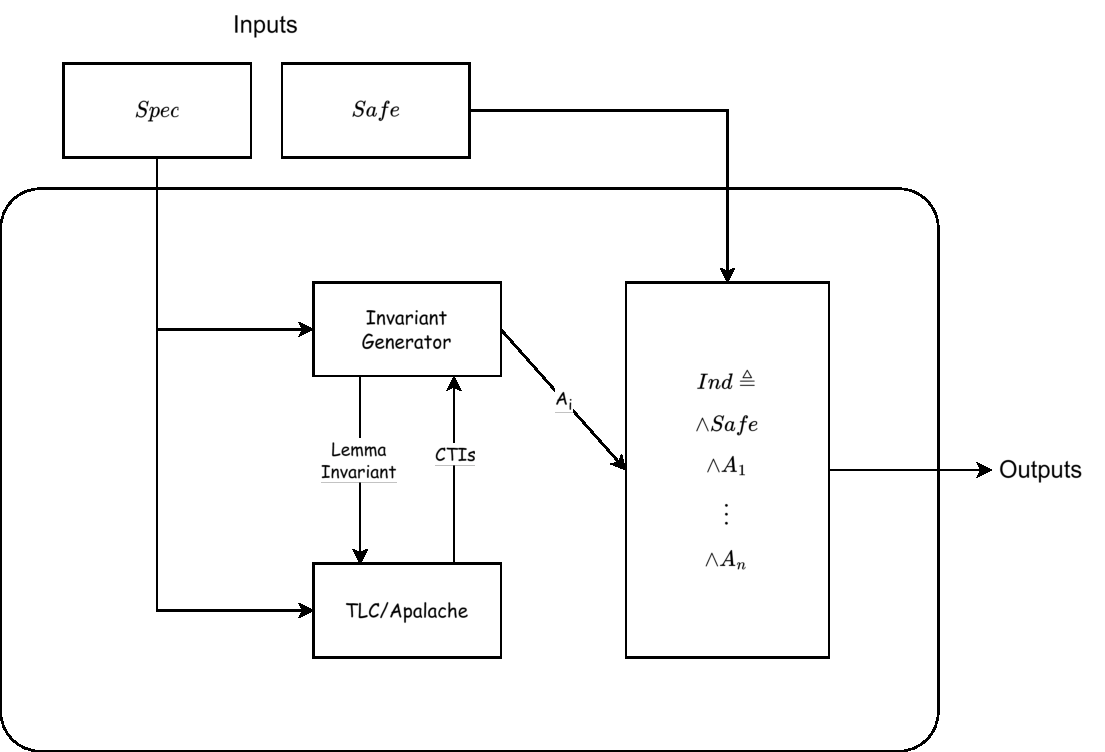
\includegraphics[width=0.7\textwidth]{figures/workflow.pdf}
    \caption{rlTLA-workflow}
    \label{fig:rltla}
\end{figure}

\begin{algorithm}[ht]
    \caption[short]{workflow of rlTLA}
    \label{alg:rltla-workflow}
    
    \begin{algorithmic}[1]
        \REQUIRE \ \\
        $M$: Finite instance of parameterized system\\
        $Safe$: Safety property
		\ENSURE \ \\
        $Ind$: Inductive Invariant Candidiate
		\STATE $Ind \gets Safe$
        \STATE $IndCTIs \gets GenrateIndCTIs(M, Ind)$
        \WHILE{$IndCTIs$ is not empty}
            \WHILE{True}
                \STATE $Inv \gets GenerateCandidateInvariant(M, IndCTIs)$
                \STATE $InvCEs \gets GenrateInvCTIs(M, Inv)$
                \IF{$InvCEs$ is not empty}
                    \STATE $Continue$
                \ENDIF
                \IF {not $CheckDeduction(Ind, Inv)$} 
                    \STATE $Ind = Ind \wedge Inv$
                    \STATE $Break$
                \ENDIF
            \ENDWHILE
            \STATE $IndCTIs \gets GenrateIndCTIs(M, Ind)$
        \ENDWHILE
        \RETURN $Ind$
    \end{algorithmic}
\end{algorithm}

\begin{align}
    Spec &\triangleq Init \wedge [Next] \\
	Spec &\vDash (s, s') \label{con:ce} \\ 
	s &\vDash  Inv \\
	s' &\nvDash  Inv 
\end{align}

基本的逻辑结构如算法\ref{alg:rltla-workflow}展示。
初始化时候,候选的归纳不变式首先析取$Safe$属性,然后基于此生成第一轮的归纳反例(Counterexample to Induction)。
在每一轮的迭代中,强化学习系统都会不断地生成一个个候选的引理不变式。
但只有满足两个条件的,才能被添加到候选归纳不变式中。
首先是,引理不变式必须,满足在运行的状态空间上是不变式,也就是没有不变式反例CE生成;
其次,新的引理不变式必须不能被已有的不变式包含,因为加入这样的引理不变式不会提高候选归纳不变式的约束能力。
这样的不变式便会加入到候选的归纳不变式中做析取,直到对候选归纳不变式生成的CTI为空,即不再有归纳反例产生。
这说明现在系统中所有生成不变式的析取结果是一个包含$Safe$属性归纳不变式,也就是得到了归纳不变式,系统选择将这个结果输出给用户。

引理\ref{con:ce}给出了不变式反例CE的定义,和归纳反例不同的是,状态$s$和$s'$都来自规约允许的允许状态,也就是图\ref{fig:ind-cti}中可到达的允许空间里的状态。

\section{候选不变式检验模块}

候选不变式检验模块需要调用模型检查器,并且需要将输出解析,并将结果返回给生成模块。
检验模块的工作,可以分为三个部分,分别是检验新生成候选不变式正确性、独立性和多个不变式析取结果的递归性。

引理\ref{con:inv_correct}表达了候选不变式的正确性,即候选不变式在规约有限实例运行的每个状态下都成立。
引理\ref{con:inv_indepence}表达了候选不变式的独立性,即新生成的候选不变式不能被已有的不变式的析取结果包含。
\begin{align}
    &Spec \vDash Inv \label{con:inv_correct} \\
    &IndCand \wedge Next \nvDash Inv \label{con:inv_indepence}
\end{align}

检验候选不变式的正确性,就是检验每个候选不变式是否在规约的每个状态下,布尔值都为真。
这个问题虽然简单,但是直觉上可能需要遍历许多状态和多个状态转移轨迹,可能需要很长的时间。
但是实际上,很多的不正确的候选不变式在规约的某个比较容易到达的状态被验证器检验出来,便可以退出了。
一个正确的不变式,尽管现在还不能成为归纳不变式,但是它确实我们需要归纳不变式的开始。

检验不变式的独立性时,我们需要验证新生成的候选不变式是否能被已有的不变式的析取结果包含。
检验不变式的独立性十分重要,尤其是对于指导强化学习生成候选不变式,
因为如果新生成的候选不变式能被已有的不变式的析取结果包含,那么生成模块为了得到更高的奖励,
会偏向于生成这样的候选不变式,这样会导致不变式的重复,析取的结果的约束能力也不能加强,对状态空间不能做出有价值的修剪,
这样的不变式便是没有意义的。系统也就无法找到一个合适的归纳不变式。
一个不被已有不变式包含的候选不变式,便可以成为一个合适的引理不变式。

检验归纳不变式的递归性,是我们工作的终点。
如果多个不变式的析取结果具有递归性,那么我们可以将这个析取结果作为归纳不变式,我们可以将这个结果输出,并结束这个循环。
对于不变式的递归性质,在引理\ref{con:init}和\ref{con:inductive}中已经提及。
归纳不变式需要包含所有的初始状态,并且,从归纳不变式约束的状态出发,进行状态转移,新生成的状态也需要满足归纳不变式。
另外,我们最根本的目的是证明安全属性,所有归纳不变式需要蕴含安全属性。

如果给出的候选不变式不正确,检验模块应当给出不变式反例,以帮助生成模块调整策略,生成正确的候选不变式。
同样的,如果当前给出的引理不变式的析取结果不是归纳不变式,检验模块还应该返回归纳反例。
不变式反例和归纳反例有着相似的内容,由两个状态组成,前一个状态满足现有的候选(归纳)不变式,而后一个状态则不满足。

\section{候选不变式生成模块}

\begin{figure}[h]
    \centering
    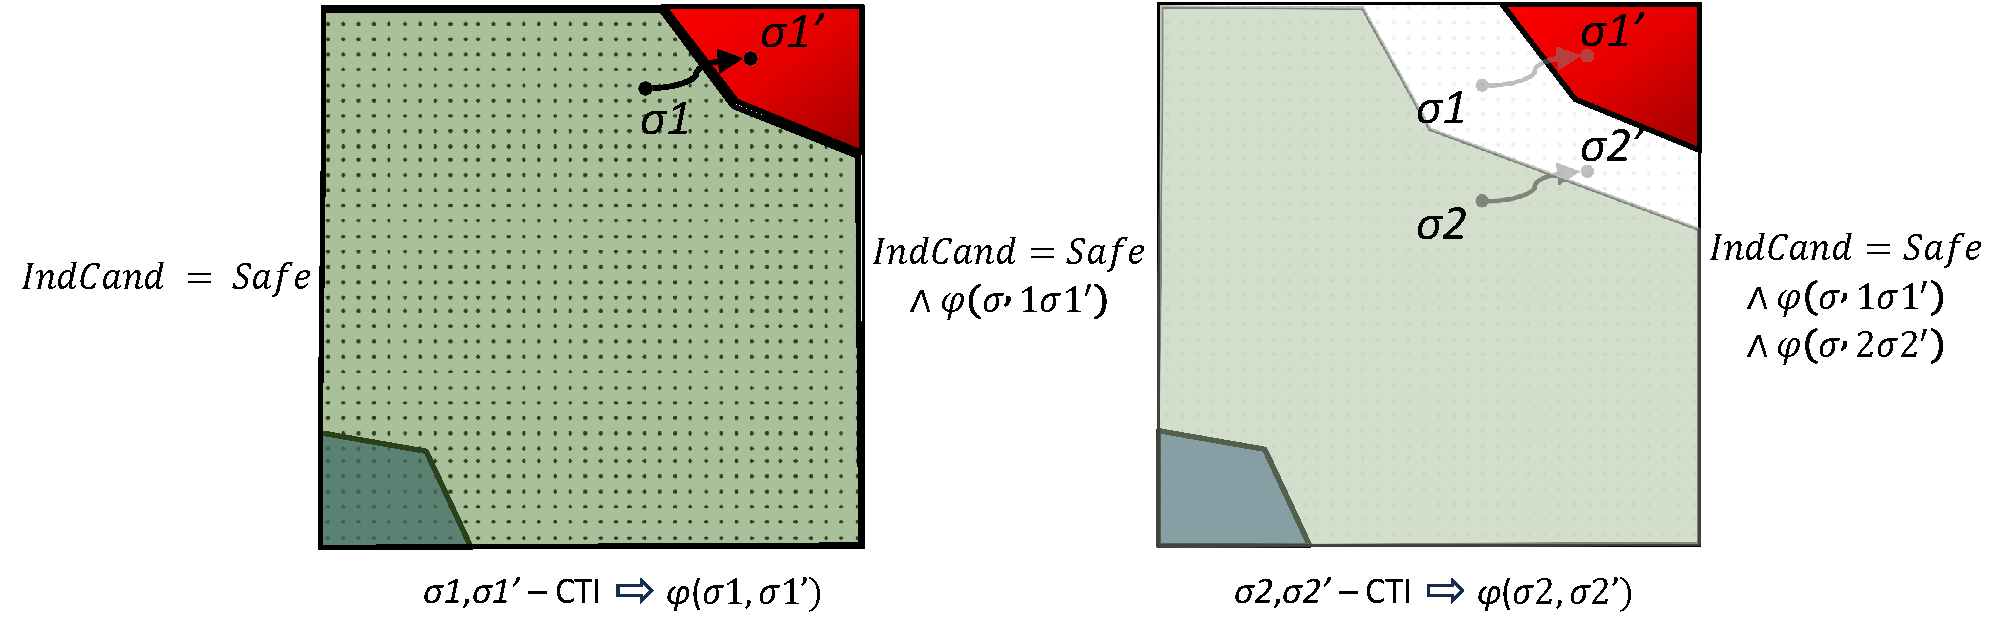
\includegraphics[width=0.95\textwidth]{figures/eliminate_cti.pdf}
    \caption{杀死归纳反例以获得归纳不变式}
    \label{fig:eliminate_cti}
\end{figure}

图\ref{fig:eliminate_cti}是一个典型的杀死归纳反例以获得归纳不变式的过程。
候选的归纳不变式初始化为$Safe$属性,然后基于此生成第一轮的归纳反例(Counterexample to Induction)。
以杀死归纳反例为目的,生成模块不断地生成一个个候选的引理不变子式。
以此迭代,直到没有归纳反例产生,也就是获得了最后的归纳不变式。
因此,归纳反例对生成归纳不变式有重要的指导作用。

这些不变式以一阶逻辑谓词的形式存在,首先需要满足在规约的有限实例上保持布尔值为真,其次便是需要杀死一些归纳反例。
为了找到这些不变式,我们使用一种基于语法合成指导的归纳不变式生成技术。
我们从输入的种子(seed)谓词中,按照强化学习模块的意愿选择一部分种子谓词,并按照语法组合成一个可能的不变式。
每个种子谓词都是针对系统状态变量的布尔表达式。
当然,我们也有可能采取给出种子谓词的否定,根据\TLA 的语法,我们只需要在给出的谓词前面加上否定符号 \textbf{“\~{}”}即可。
这部分的决定权交给强化学习模块,强化学习模块会根据当前的状态,选择一个合适的种子谓词,或者它的否定。

一个不变式的语法大致可以表达为:
\begin{align}
    <lemma> &: = <quant>:<expr>   \\
    <quant> &:= \forall x\ \backslash in\ SetA | \exists y\ \backslash in\ SetB \\
    <expr>  &:= <seed>| \sim<seed> | <seed> \lor <seed>
\end{align}
注意到,我们对于引理不变式内部每个谓词之间的连接方式统一选择了合取符号“$\lor$”。
这是因为,一方面这种语法在表达归纳不变已经足够完备\cite{or-complete},
在每个引理不变式内部使用合取计算,对引理不变式之间选择析取计算足够我们表达对于绝大多数规约的归纳不变式;
另一方面,由于简化了种子谓词之间的逻辑计算方式,不再需要对此分别研究,也可以帮助了我们简化问题,缩小了搜索不变式的空间。
另外,对于每个引理不变式的量词部分,我们统一使用了直接的输入。
这部分量词,往往和后面跟随的谓词逻辑表达式有关系,而这部分输入又来自于用户设置的种子谓词。
因此,直接使用和种子谓词匹配好的量词表达式,避免了许多无意义的候选不变式,方便了对候选不变式的生成。
有些时候,可能量词表达式中定义的变量在后面的谓词逻辑表达式中并没有使用,但这不影响生成的结果的布尔值,对于这部分多余的量词定义,可以不做处理。


\section{强化学习在生成模块中的应用}

本文的目的是希望研究强化学习在自动的归纳不变式生成过程中的应用。
强化学习是一种通过智能体和环境的交互,智能体通过观察环境的状态,采取行动,获得奖励,来学习如何在环境中获取最大的奖励。
对于归纳不变式生成问题而言,智能体可以根据环境的变化,连续地进行动作选择的,并根据环境返回的奖励值,来调整策略的特点,可以加速归纳不变式的生成过程。

强化学习模块接受\TLA 协议和检验模块对于本身生成的候选不变式的检验结果,修改策略,生成更加合理的候选不变式。
强化学习模块的输入是一个状态,输出是一个动作,动作是对于种子谓词的选择与否,和是否选择它的否定。

强化学习模块的目标是生成一个合适的引理不变式,这个引理不变式在规约的每个状态下都成立,且不会被已有的不变式的析取结果包含。
这个过程是自动化的,但人可以通过调整对强化学习智能体在每个状态下的每个动作的选择给出合适的奖励或者惩罚,以指导智能体学习到
一个合适的策略并不断调整,以应用到后续的候选不变式生成中。

环境对智能体的动作给出反馈,包括奖惩值和自身的状态信息。

最高的奖励应当给予给出最终的归纳不变式的行为,也就是给出了一个不变式,使得它和前面所有不变式的析取结果是归纳不变式的行为。
当强化学习模块给出一个不变式的时候,也应当给出一定的奖励。给出一个不变式,尤其是给出第一个不变式,往往是一个十分困难的过程。
而且,这一步也是实现最终目标的关键。因此,我们应当给予一定的奖励,以鼓励智能体继续学习。
生成一个已经被已有不变式包含的不变式,尽管没有意义,但也体现出智能体如何寻找不变式的能力,因此也应当给予一定的奖励。
这个奖励的值很小,但是也是必要的。因为这个过程是一个逐步的过程,智能体需要不断地尝试,才能找到一个合适的不变式。
但是,为了防止智能体的惰性,我们不允许智能体在已有的不变式上简单的合取上一个谓词,然后给出这个谓词作为候选不变式,
同样的,不允许在一个错误的不变式上去除掉一些谓词,以得到候选不变式。
这是简单的重复,是没有意义的,我们对智能体的这种行为应当给予惩罚。

环境的状态信息包括候选归纳不变式中已有的引理不变式,归纳反例,种子谓词,以及规约的状态信息,在强化学习给出的候选不变式不正确时,
也应当给出在哪些状态下,这个候选不变式的布尔值为假,以便于智能体基于错误的候选不变式做出调整。

\section{非功能设计}

因为逻辑复杂,运行时间长,为了开发人员和用户对系统信息可见,需要设计有日志模块,以不同的日志等级记录系统的运行状态。
日志模块应当在系统运行的每个重要步骤打印具体的运行信息,同时在系统出现运行错误时,打印错误信息,以便开发人员定位错误进行调试。

为了研究和评估系统的性能,需要设计计时模块,记录系统运行的时间,以便于后续的性能分析。同时,需要在循环中记录强化学习模块的特征信息。
